\documentclass[professionalfonts]{beamer}
%
% Choose how your presentation looks.
%
% For more themes, color themes and font themes, see:
% http://deic.uab.es/~iblanes/beamer_gallery/index_by_theme.html
%
\mode<presentation>
{
  \usetheme{Luebeck}      % or try Darmstadt, Madrid, Warsaw, ...
  \usecolortheme{whale} % or try albatross, beaver, crane, ...
  \usefonttheme{serif}  % or try serif, structurebold, ...
  \setbeamertemplate{navigation symbols}{}
  \setbeamertemplate{caption}[numbered]
  \setbeamertemplate{page number in head/foot}[totalframenumber]
  \setbeamertemplate{headline}{}
} 

%%%%%%%%%%%%%%%%%%%%%%%%%%%%%%%%%%%%%%%%%%%%%%
%Include any other add-on  packages you need:%
%%%%%%%%%%%%%%%%%%%%%%%%%%%%%%%%%%%%%%%%%%%%%%
\usepackage{amsmath,graphicx,mathtools, amssymb}
\allowdisplaybreaks
\usepackage{booktabs} % Required for better horizontal rules in tables
\usepackage{listings} % Required for insertion of code
\usepackage[utf8]{inputenc}
\usepackage[T1]{fontenc}
\usepackage{lmodern}
\usepackage[labelfont=bf,labelsep=period]{caption}
\usepackage{multirow}
\usepackage{textcomp}
\usepackage{hyperref}
\usepackage{afterpage}
\usepackage{pdflscape}
\usepackage{hhline}
%\usepackage{enumitem}
\usepackage{bm}
\usepackage{datetime}
\usepackage{xstring} % conditionals
\usepackage{xcolor}
\usepackage{movie15}
\usepackage{bm}
\usepackage{natbib}

\title[Dissertation defence]{New quantum computing techniques applied to chemistry dynamics}
\author{Lucas Ramos Cardoso Tin\^{o}co Cortez}
\institute{Texas Tech University}
\date{\today}

%%%%%%%%%%%%%%%%%%%%%%%%%%%%%%%%%%%%%%%%%%%%%%%
%Uncomment if the grad school doesn't like the%
%line under the  running head:                %
%%%%%%%%%%%%%%%%%%%%%%%%%%%%%%%%%%%%%%%%%%%%%%%
%\renewcommand{\headrulewidth}{0pt}


%%%%%%%%%%%%%%%%%%%%%%%%%%%%%%%%%%%%%%%%%%%%%%%%%%
%Spacing -- Do you want double or one-and-a-half?%
%%%%%%%%%%%%%%%%%%%%%%%%%%%%%%%%%%%%%%%%%%%%%%%%%%
%\doublespacing
%\onehalfspacing
%%%%%%%%%%%%%%%%%%%%%%%%%%%%%%%%%%%%%%%%%%%%%%%%%%%%%%%%%%%%%
%Leave the one you want uncommented.                        %
%In places where single-line-spacing is appropriate         %
%e.g, extended quotations, you can enclose the material     %
%in a singlespacing environment (with \begin{singlespacing} %
% ...  \end{singlespacing}                                  %
%%%%%%%%%%%%%%%%%%%%%%%%%%%%%%%%%%%%%%%%%%%%%%%%%%%%%%%%%%%%%


%%%%%%%%%%%%%%%%%%%%%%%%%%%%%%%%%%%%%%%%%%%%%%%%%%
%Other preamble stuff, e.g., theorem environments%
%or newcommands go here:                         %
% e.g.                                           %
%%%%%%%%%%%%%%%%%%%%%%%%%%%%%%%%%%%%%%%%%%%%%%%%%%
% \newtheorem{theorem}{Theorem}
% \newtheorem{proposition}[theorem]{proposition}
% \newtheorem{question}{Question}
% \newtheorem{conjecture}{Conjecture}
%\newcommand\Set[2]{\left\{\,#1\middle\mid#2\,\right\}}
\newcommand{\bx}{\bm{x}}
\newcommand{\br}{\bm{r}}
\newcommand{\bra}[1]{\ensuremath{\left\langle#1\right\vert}}
\newcommand{\ket}[1]{\ensuremath{\left|#1\right\rangle}}
\newcommand{\braket}[2]{\left< #1 \middle\vert #2 \right>}
\newcommand{\sandwich}[3]{\left< #1 \middle\vert #2 \middle\vert #3 \right>}
%\newcommand{\norm}[1]{\left\lVert #1 \right\rVert}
%\newcommand{\abs}[1]{\lVert #1 \rVert}
\newcommand{\inpr}[1]{\left< #1 \right>}
\newcommand{\s}[1]{\sin\left( #1 \right)}
\newcommand{\ssq}[1]{\sin^2\left( #1 \right)}
\newcommand{\co}[1]{\cos\left( #1 \right)}
\newcommand{\cosq}[1]{\cos^2\left( #1 \right)}
\newcommand{\av}[1]{\left< #1 \right>}
\newcommand{\her}[2]{H_{#1}\left( #2 \right)}
\newcommand{\herv}[1]{H_{\nu}\left( #1 \right)}
%\renewcommand{\labelenumi}{\Roman{enumi} -}
\newcommand{\ex}[1]{\exp\left( #1 \right)}
\newcommand{\closepar}{)}
\newcommand{\paren}[1]{\left( #1 \right)}
\newcommand{\ddx}{\frac{d}{dx}}
\newcommand{\ddt}{\frac{d}{dt}}
\newcommand{\pdx}{\frac{\partial}{\partial x}}
\newcommand{\pdt}{\frac{\partial}{\partial t}}
\newcommand{\dd}[1]{\frac{d}{d#1}}
\newcommand{\pd}[1]{\frac{\partial}{\partial #1}}
\newcommand{\fpd}[2]{\frac{\partial #1}{\partial #2}}
\newcommand{\pp}[1]{\frac{\partial \Psi}{\partial #1}}
\newcommand{\kpp}[1]{\frac{\partial \ket\Psi}{\partial #1}}
\newcommand{\bpp}[1]{\frac{\partial \bra\Psi}{\partial #1}}
\newcommand{\kppn}[2]{\frac{\partial^{#2} \ket\Psi}{\partial {#1}^{#2}}}
\newcommand{\bppn}[2]{\frac{\partial^{#2} \bra\Psi}{\partial {#1}^{#2}}}
\newcommand{\kppd}[2]{\frac{\partial^{2} \ket\Psi}{\partial #1 \partial #2}}
\newcommand{\bppd}[2]{\frac{\partial^{2} \bra\Psi}{\partial #1 \partial #2}}
\newcommand{\ddn}[2]{\frac{d^{#1}}{d#2^{#1}}}
\newcommand{\pdn}[2]{\frac{\partial^{#1}}{\partial#2^{#1}}}
%\newcommand{\orb}{N}
%\newcommand{\elec}{n}
\newcommand{\elec}{N}
\newcommand{\nuc}{N_{N}}
\newcommand{\orb}{K}
\newcommand{\Ld}[1]{\hat L_{#1}}
\newcommand{\anio}[1]{a_{\oo{#1}}}
\newcommand{\aniu}[1]{a_{\uo{#1}}}
\newcommand{\anig}[1]{a_{\go{#1}}}
\newcommand{\creo}[1]{a^\dagger_{\oo{#1}}}
\newcommand{\creu}[1]{a^\dagger_{\uo{#1}}}
\newcommand{\creg}[1]{a^\dagger_{\go{#1}}}
\newcommand{\vac}{\ket{vac}}
\newcommand{\anticom}[2]{\left\{ #1, #2 \right\}}
\newcommand{\ind}[1]{{\uo #1 \oo #1}}
\newcommand{\Paulid}[1]{
		\IfEqCase{#1}{
			{ii}{I \otimes I}
			{ix}{I \otimes X}
			{iy}{I \otimes Y}
			{iz}{I \otimes Z}
			{xi}{X \otimes I}
			{xx}{X \otimes X}
			{xy}{X \otimes Y}
			{xz}{X \otimes Z}
			{yi}{Y \otimes I}
			{yx}{Y \otimes X}
			{yy}{Y \otimes Y}
			{yz}{Y \otimes Z}
			{zi}{Z \otimes I}
			{zx}{Z \otimes X}
			{zy}{Z \otimes Y}
			{zz}{Z \otimes Z}
		}[\PackageError{p2d}{Undefined option to uo: #1}{}]
}
\newcommand{\uo}[1]{
		\IfEqCase{#1}{
			{0}{\mu}
			{1}{\nu}
			{2}{\xi}
		}[\PackageError{uo}{Undefined option to uo: #1}{}]
}
\newcommand{\oo}[1]{
		\IfEqCase{#1}{
			{0}{\alpha}
			{1}{\beta}
			{2}{\gamma}
		}[\PackageError{unocorb}{Undefined option to unuo: #1}{}]
}
\newcommand{\go}[1]{
		\IfEqCase{#1}{
			{0}{\zeta}
			{1}{\eta}
			{2}{\iota}
			{3}{\kappa}
		}[\PackageError{unocorb}{Undefined option to go: #1}{}]
}
\newcommand{\psiu}[1]{
	\psi_{\uo{#1}}
}
\newcommand{\psio}[1]{
	\psi_{\oo{#1}}
}
\newcommand{\psig}[1]{
	\psi_{\go{#1}}
}

\newcommand{\X}{\begin{bmatrix}	0 & 1 \\ 1 & 0 \end{bmatrix} }
\newcommand{\Y}{\begin{bmatrix}	0 & -i \\ i & 0 \end{bmatrix} }
\newcommand{\Z}{\begin{bmatrix}	1 & 0 \\ 0 & -1 \end{bmatrix} }
\newcommand{\I}{\begin{bmatrix}	1 & 0 \\ 0 & 1 \end{bmatrix} }
\newcommand{\Phase}[1]{\begin{bmatrix} 1 & 0 \\ 0 & e^{i#1} \end{bmatrix} }
\newcommand{\nPhase}[1]{\begin{bmatrix} 1 & 0 \\ 0 & e^{-i#1} \end{bmatrix} }
\newcommand{\II}{\begin{bmatrix}
1 & 0 & 0 & 0 \\
0 & 1 & 0 & 0 \\
 0 & 0 & 1 & 0 \\
0 & 0 & 0 & 1
\end{bmatrix}}
\newcommand{\IX}{ \begin{bmatrix}
0 & 1 & 0 & 0 \\
1 & 0 & 0 & 0 \\
 0 & 0 & 0 & 1 \\
0 & 0 & 1 & 0
\end{bmatrix}}
\newcommand{\IY}{ \begin{bmatrix}
0 & -i & 0 & 0 \\
i & 0 & 0 & 0 \\
 0 & 0 & 0 & -i \\
0 & 0 & i & 0
\end{bmatrix}}
\newcommand{\IZ}{ \begin{bmatrix}
1 & 0 & 0 & 0 \\
0 & -1 & 0 & 0 \\
 0 & 0 & 1 & 0 \\
0 & 0 & 0 & -1
\end{bmatrix}}
\newcommand{\XI}{ \begin{bmatrix}
0 & 0 & 1 & 0 \\
0 & 0 & 0 & 1 \\
 1 & 0 & 0 & 0 \\
0 & 1 & 0 & 0
\end{bmatrix}}
\newcommand{\XX}{ \begin{bmatrix}
0 & 0 & 0 & 1 \\
0 & 0 & 1 & 0 \\
 0 & 1 & 0 & 0 \\
1 & 0 & 0 & 0
\end{bmatrix}}
\newcommand{\XY}{ \begin{bmatrix}
0 & 0 & 0 & -i \\
0 & 0 & i & 0 \\
 0 & -i & 0 & 0 \\
i & 0 & 0 & 0
\end{bmatrix}}
\newcommand{\XZ}{ \begin{bmatrix}
0 & 0 & 1 & 0 \\
0 & 0 & 0 & -1 \\
 1 & 0 & 0 & 0 \\
0 & -1 & 0 & 0
\end{bmatrix}}
\newcommand{\YI}{ \begin{bmatrix}
0 & 0 & -i & 0 \\
0 & 0 & 0 & -i \\
 i & 0 & 0 & 0 \\
0 & i & 0 & 0
\end{bmatrix}}
\newcommand{\YX}{ \begin{bmatrix}
0 & 0 & 0 & -i \\
0 & 0 & -i & 0 \\
 0 & i & 0 & 0 \\
i & 0 & 0 & 0
\end{bmatrix}}
\newcommand{\YY}{ \begin{bmatrix}
0 & 0 & 0 & -1 \\
0 & 0 & 1 & 0 \\
 0 & 1 & 0 & 0 \\
-1 & 0 & 0 & 0
\end{bmatrix}}
\newcommand{\YZ}{ \begin{bmatrix}
0 & 0 & -i & 0 \\
0 & 0 & 0 & i \\
 i & 0 & 0 & 0 \\
0 & -i & 0 & 0
\end{bmatrix}}
\newcommand{\ZI}{ \begin{bmatrix}
1 & 0 & 0 & 0 \\
0 & 1 & 0 & 0 \\
 0 & 0 & -1 & 0 \\
0 & 0 & 0 & -1
\end{bmatrix}}
\newcommand{\ZX}{ \begin{bmatrix}
0 & 1 & 0 & 0 \\
1 & 0 & 0 & 0 \\
 0 & 0 & 0 & -1 \\
0 & 0 & -1 & 0
\end{bmatrix}}
\newcommand{\ZY}{ \begin{bmatrix}
0 & -i & 0 & 0 \\
i & 0 & 0 & 0 \\
 0 & 0 & 0 & i \\
0 & 0 & -i & 0
\end{bmatrix}}
\newcommand{\ZZ}{ \begin{bmatrix}
1 & 0 & 0 & 0 \\
0 & -1 & 0 & 0 \\
 0 & 0 & -1 & 0 \\
0 & 0 & 0 & 1
\end{bmatrix}}
\DeclarePairedDelimiter\norm{\lVert}{\rVert}
\DeclarePairedDelimiter\abs{\lvert}{\rvert}

%Presentation macros:
\newcommand{\SubItem}[1]{
    {\setlength\itemindent{15pt} \item[*] #1}
}

%Transition for every section
\AtBeginSection[]
{
  \begin{frame}
    \frametitle{Table of Contents}
    \tableofcontents[currentsection]
  \end{frame}
}


\begin{document}

\begin{frame}
	\titlepage
\end{frame}
%%%%%%%%%%%%%%%%%%%
%End of title page%
%%%%%%%%%%%%%%%%%%%

\begin{frame}
\tableofcontents	%Leave this here (table will auto-update as you write new sections/subsubsections/appendix)
\end{frame}

\section{\textbf{Introduction}}
\subsection{\textbf{What is Quantum Computing}}

\begin{frame}{Classical Computer}
\begin{figure}[b]
	\centering
	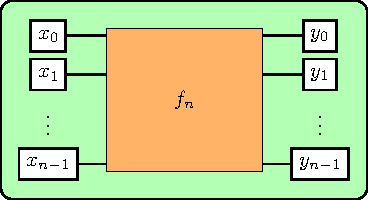
\includegraphics[width=0.75\textwidth]{img/classical}
\end{figure}
	\begin{itemize}
		\item $x_i$ and $y_i$ are states of a 2-level classical system \{0, 1\}, bits
		\item Two equivalent models: Turing machine and circuit model
	\end{itemize}
\end{frame}

\begin{frame}{Quantum Computer}
\begin{figure}[b]
	\centering
	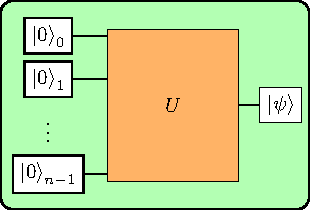
\includegraphics[width=0.75\textwidth]{img/quantum}
\end{figure}
	\begin{itemize}
		\item $\ket 0_i$ are states of a 2-level quantum system $\{\ket 0, \ket 1\}$, qubits
		\item One majorly used model: Circuit model
	\end{itemize}
\end{frame}

\begin{frame}{Quantum Computing}
	\begin{itemize}
		\item States are vectors in a 2-dimensional Hilbert space over $\mathbb{C}$
		\item Bases of the Hilbert space are orthonormal
			\SubItem {Most usual is 
				$\left\{
					\ket 0 = \begin{bmatrix} 1 \\ 0 \end{bmatrix},
					\ket 1 = \begin{bmatrix} 0 \\ 1 \end{bmatrix}
				\right\}$}
		\item We write the state of a qubit $\ket \phi$ as $\ket \phi = \alpha_0 \ket 0 + \alpha_1 \ket 1$
			\SubItem {$\alpha_i \in \mathbb{C}$}
			\SubItem {$\norm {\alpha_0}^2 + \norm{\alpha_1}^2 = 1 $}
			\SubItem {Measuring $\ket \phi$ yields $\ket 0$ or $\ket 1$, with probability $\norm{\alpha_i}^2$}
			\SubItem {Unitary operators are necessary to mantain these properties}
	\end{itemize}
\end{frame}

\subsection{\textbf{Quantum Advantages}}
\begin{frame}{Quantum advantages}
	\begin{itemize}
		\item Quantum systems cannot be efficiently simulated on classical computers \citep{feynman}, requiring exponential complexity
		\SubItem{There are quantum algorithms \citep{quantumsimulation} that attain exponential speedups}
		\item Other problems for which quantum computers attain exponential speedups are:
			\SubItem{Factorization \citep{shor}}
			\SubItem{Solving systems of linears equations \citep{harrow}}
	\end{itemize}
\end{frame}

\subsection{\textbf{Challenges in Quantum Computing}}

\cite{moorequantum}
\cite{ibmblog}
\cite{dyanokov}
\begin{frame}{Challenges in Quantum Computing}
	\begin{itemize}
		\item Quantum systems cannot be efficiently simulated on classical computers \citep{feynman}, requiring exponential complexity
		\SubItem{There are quantum algorithms \citep{quantumsimulation} that attain exponential speedups}
		\item Other problems for which quantum computing attains exponential speedups are:
			\SubItem{Factorization \citep{shor}}
			\SubItem{Solving systems of linears equations \citep{harrow}}
	\end{itemize}
\end{frame}

\section{\textbf{Background}}

\begin{frame}{Overview flowchart}
\begin{figure}[b]
	\centering
	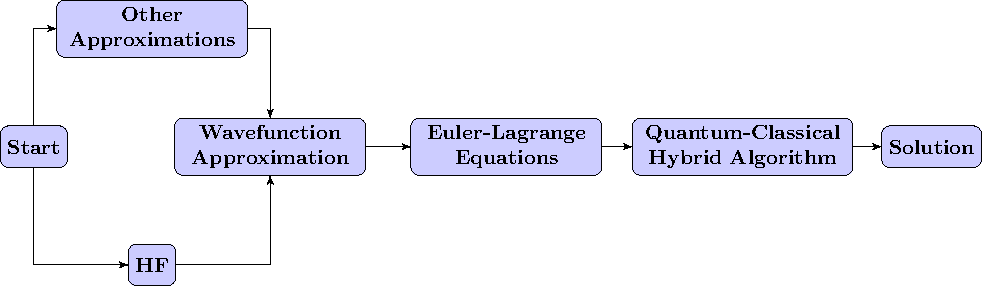
\includegraphics[width=\textwidth]{../flowcharts/flowchart2}
\end{figure}
\end{frame}

\begin{frame}{TDVP flowchart}
\begin{figure}[b]
	\centering
	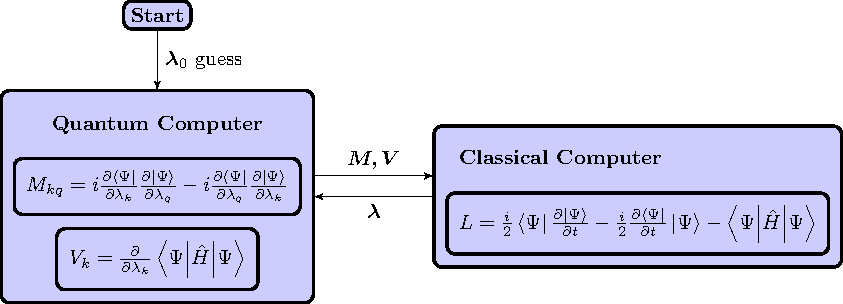
\includegraphics[width=\textwidth]{../img/variation_figure}
\end{figure}
\end{frame}

\subsection{\textbf{Quantum Chemistry: Second quantization}}

\begin{frame}{The system}
	\begin{itemize}
		\item $\elec$ electrons
		\item $\orb$ orthonormal spin orbitals ($\orb \geq \elec$)
		\item $\{\oo{0}, \oo{1}, \oo{2}, \ldots\}$ index occupied(hole) orbitals
		\item $\{\uo{0},\uo{1},\uo{2}, \ldots\}$ index unoccupied(particle) orbitals
		\item $\{\go{0}, \go{1}, \go{2}, \go{3}, \ldots\}$ index orbitals in general.
	\end{itemize}
\end{frame}

\begin{frame}{Other considerations}
	\begin{itemize}
		\item Nuclei at rest when calculating the electron dynamics
		\item Wavefunction for each orbital: $\psig 0(\mathbf{x}_1)$, where $\bx_1 = \paren{\br_1, \sigma_1}$
			\SubItem {$\br_1$ spatial coordinate}
			\SubItem {$\sigma_1$ spin coordinate}
		\item Creation $\creg{0}$ and annihilation $\anig{0}$ operator
		\item vacuum state $\vac$
	\end{itemize}
\end{frame}

\begin{frame}{Creation and annihilation operators}
	\begin{itemize}
		\item $\creg 0 \vac = \ket{\psig 0}$
		\item $\creg 0 \creg 1 \vac = \creg 0 \ket{\psig 1} = \ket{\psig 0\psig 1}$
		\item $\creg 1 \creg 0 \vac = \creg 1 \ket{\psig 0} = \ket{\psig 1\psig 0} = - \ket{\psig 0\psig 1} = -\creg 0 \creg 1 \vac$
		\item $\anig 0 \vac = 0$
		\item $\anig 0 \ket{\psig 0}  = \vac $
		\item Anti-commutation relationships:
			\SubItem{$\anticom{\creg 0}{\anig 1} = \delta_{\go 0 \go 1}$}
			\SubItem{$\anticom{\creg 0}{\creg 1} = \anticom{\anig 0}{\anig 1} = 0$}
	\end{itemize}
\end{frame}

\begin{frame}
	\begin{itemize}
		\item Wavefunction with only occupied orbitals:
			\SubItem{$
				\ket\Psi 
				= \creo 0 \creo 1 \ldots a^\dagger_{\elec} \vac 
				= \ket {\psio 0 \psio 1 \ldots \psi_\elec} 
				= \det \left[\psio 0(\bx_i)\right]
			$}
		\item Single excited states:
			\SubItem{$
				\ket {\Psi_{\oo 0}^{\uo 0}}
				= \creu 0 \anio 0 \ket\Psi 
				= \ket{\psiu 0 \psio 1 \ldots \psi_\elec} 
			$}
		\item Double excited states:
			\SubItem{$
				\ket {\Psi_{\oo 0 \oo 1}^{\uo 0 \uo 1}}
				= \creu 1 \anio 1 \creu 0 \anio 0 \ket\Psi 
				= \ket{\psiu 0 \psiu 1 \psio 2 \ldots \psi_\elec} 
			$}
		\item Hamiltonian:
			\SubItem{$
				\hat H_e = \sum_{\go 0, \go 1}h_{\go 0 \go 1}\creg 0 \anig 1 + 
				\frac 1 4 \sum_{\go 0, \go 1, \go 2, \go 3} \sandwich{\go 0 \go 1}{}{\go 2 \go 3}\creg 0 \creg 1 \anig 2 \anig 3
			$}
			\SubItem{$
				h_{\go 0 \go 1} 
				= \sandwich {\go 0} {h} {\go 1} 
				= \int\psig 0^*(\bx_1)h(\br_1)\psig 1(\bx_1)d\bx_1 
			$}
			\SubItem{$
				\sandwich{\go 0 \go 1}{}{\go 2 \go 3}
				= \braket{\go 0 \go 1}{\go 2 \go 3} - \braket{\go 0 \go 1}{\go 3 \go 2}
			$}
			\SubItem{$
				\braket{\go 0 \go 1}{\go 2 \go 3}
				= \iint
				\psig 0^*(\bx_1)\psig 2(\bx_1) 
				\frac 1 {r_{12}}
				\psig 1^*(\bx_2)\psig 3(\bx_2) 
				d\bx_1 d\bx_2 
			$}
			\SubItem{$h(\br_1)$ is the $1e^-$ Hamiltonian and $\frac 1 {r_{12}}$ is the Coulomb repulsion operator}
	\end{itemize}
\end{frame}

\subsection{\textbf{Lie Algebras}}

\begin{frame}{Lie Algebras}
	\begin{itemize}
		\item $\orb^2$ elements in $Alg(\{\creg 1 \anig 0\}) \subset U(\orb)$
			\SubItem{Group $U(\orb)$ generated by all pair operators $\{\creg 0 \anig 1 \}$}
		%
		\item $\elec^2$ elements in $Alg(\{\creo 1 \anio 0\}) \subset U(\elec) \subset U(\orb)$
			\SubItem{Mixes holes with holes}
		\item $(\orb - \elec)^2$ elements in $Alg(\{\creu 1 \aniu 0\}) \subset U(\orb - \elec) \subset U(\orb)$
			\SubItem{Mixes particles with particles}
			\SubItem{$\left[\creo 0 \anio 1, \creu 0 \aniu 1\right] = 0$}
			\SubItem{$\implies {U(\elec) \cap U(\orb - \elec) = 0}$}
	\end{itemize}
\end{frame}

\subsection {\textbf{Fukutome Unitary Approach to HF Theory}}

\begin{frame}{Fukutome}
	\begin{itemize}
		\item $U(\orb) = U(\elec) \oplus_d U(\orb - \elec)$
			\SubItem{
			\(
				\hat U(\bm u) = 
				\hat U(\bm u_\xi) \cdot 
				\hat U(\bm u_\lambda) \implies 
				\bm u = 
				\bm u_\xi \cdot 
				\bm u_\lambda
				\)
			}
		\item Their actions on the reference Slater determinant state are:
			\SubItem{
				\(
					\hat U(\bm u_\xi) \ket\Psi
					= \det(\bm w)\ket\Psi \sim \ket \Psi
				\)
			}
			\SubItem{
				\(
					\hat U(\bm u_\lambda) \ket\Psi
					= \ket\Phi
				\)
			}
	\end{itemize}
\end{frame}

\section{\textbf{Methodology}}\label{chap:methodology}

\subsection{\textbf{Obtaining wavefunction}}

\begin{frame}{Considerations}
	\begin{itemize}
		\item $\elec = 2$, $\orb = 4$
		\item Use HF to obtain wavefunction $\ket\Psi = \bm u_\lambda \ket 0$.
		\item Since opposite spin orbitals don't interact:
			\( u_\lambda
			= \bigotimes_{\uo 0 \oo 0} u_{\lambda_{\uo 0 \oo 0}}
			\)
		\SubItem{\(
			\bm u_{\lambda_{\uo 0 \oo 0}} 
			= \begin{bmatrix}
				\bm C(\lambda_{\uo 0 \oo 0}) & 
				\bm -\bm S^\dagger(\lambda_{\uo 0 \oo 0}) \\ 
				\bm S(\lambda_{\uo 0 \oo 0}) & 
				\tilde {\bm C}(\lambda_{\uo 0 \oo 0})
			\end{bmatrix} \in \mathbb{\bm C}^{2\times 2}
			\)}
			\SubItem{$\bm u_{\lambda_\ind 0}$ acts on a single qubit}
		\SubItem{\(
				S(\lambda_\ind 0) 
				= \paren{\frac{\lambda_\ind 0}{\lambda_\ind 0^*}}^\frac 1 2\s{\abs{\lambda_\ind 0}} 
			\)}
		\SubItem{\(
				S^\dagger({\lambda_\ind 0}) 
				= \paren{\frac{\lambda_\ind 0^*}{\lambda_\ind 0}}^\frac 1 2\s{\abs{\lambda_\ind 0}} 
			\)}
		\SubItem{\(
				C(\lambda_\ind 0) 
				= \co {\abs{\lambda_\ind 0}} 
			\)}
		\SubItem{\(
				\tilde C({\lambda_\ind 0}) 
				= \co {\abs{\lambda_\ind 0}} 
			\)}
	\end{itemize}
\end{frame}

\begin{frame}{Decomposition}
	\begin{itemize}
		\item	\(\bm u_{\lambda_\ind 0} 
			= \begin{bmatrix}
				\co{\rho_\ind 0} & -e^{-i\omega_\ind 0}\s{\rho_\ind 0} \\
				e^{i\omega_\ind 0}\s{\rho_\ind 0} &  \co{\rho_\ind 0}
			\end{bmatrix} \)
		\SubItem {$\rho_\ind 0 = \abs{\lambda_\ind 0}$}
		\SubItem {$\omega_\ind 0 = \arg \lambda_\ind 0$}
	\end{itemize}

			\begin{equation*}
				\begin{split}
					&\bm u_{\lambda_\ind 0}
					= R_z(\omega_\ind 0)R_y(2\rho_\ind 0)R_z(-\omega_\ind 0) \\
					&= \begin{bmatrix}
						e^{-i\frac {\omega_\ind 0} 2} & 0 \\
						0 &  e^{i\frac {\omega_\ind 0} 2}
					\end{bmatrix} \cdot
					\begin{bmatrix}
						\co{\rho_\ind 0} & -\s{\rho_\ind 0} \\
						\s{\rho_\ind 0} &  \co{\rho_\ind 0}
					\end{bmatrix} \cdot
					\begin{bmatrix}
						e^{i\frac {\omega_\ind 0} 2} & 0 \\
						0 &  e^{-i\frac {\omega_\ind 0} 2}
					\end{bmatrix} \\
					& = 
					\co {\rho_\ind 0} I
					- i \s {\rho_\ind 0} \co{\omega_\ind 0} Y 
					+ i \s {\rho_\ind 0} \s{\omega_\ind 0} X
				\end{split}
			\end{equation*}
\end{frame}

\begin{frame}{The wavefunction}
\begin{equation*}
	\begin{split}
	\ket \Psi 
	&= \bm u_{\lambda_\ind 0} \bm u_{\lambda_\ind 1} \ket {\bar 0} \\
	&= \paren{\co {\rho_\ind 0} \ket {\psi_{\oo 0}} + e^{i\omega_\ind 0}\s {\rho_\ind 0} \ket {\psi_{\uo 0}}} \\
	& \quad \otimes \paren {\co {\rho_\ind 1} \ket {\psi_{\oo 1}} + e^{i\omega_\ind 1}\s {\rho_\ind 1} \ket {\psi_{\uo 1}}} \\
	&= \co {\rho_\ind 0 }\co {\rho_\ind 1}\ket {\psi_{\oo 0}\psi_{\oo 1}} \\
	&\quad + e^{i\omega_\ind 1}\co {\rho_\ind 0 }\s {\rho_\ind 1}\ket {\psi_{\oo 0}\psi_{\uo 1}} \\
	&\quad + e^{i\omega_\ind 0 }\s {\rho_\ind 0 }\co {\rho_\ind 1}\ket{\psi_{\uo 0} \psi_{\oo 1}} \\
	&\quad + e^{i\omega_\ind 0 }e^{i\omega_\ind 1}\s {\rho_\ind 0 }\s {\rho_\ind 1}\ket{\psi_{\uo 0} \psi_{\uo 1}} 
	\end{split}
\end{equation*}
\end{frame}

%-------------------------------------------------------------------------------------

\subsection {\textbf{Dynamics}}

\begin{frame}{Lagrangian equations}
	\begin{itemize}
		\item Lagrangian:
		\(
	L = \frac{\sandwich{\Psi(t)}{\frac{i}{2}\left(\overrightarrow{\pd t} - \overleftarrow{\pd t}\right) - \hat H}{\Psi(t)}}{\braket{\Psi(t)}{\Psi(t)}}
			\)
			\SubItem{$\Psi$ is normalized: $\braket \Psi \Psi = 1$}
			\SubItem{\(
				{\kpp t} = \kpp {\rho_\ind 0 }\dot \rho_\ind 0
	+	\kpp {\omega_\ind 0}\dot \omega_\ind 0
	+	\kpp {\rho_\ind 1 }\dot \rho_\ind 1
	+	\kpp {\omega_\ind 1}\dot \omega_\ind 1
			\)}
			\SubItem{We need to take $\kpp{x}$, $x \in \{\omega_\ind 1, \omega_\ind 0, \rho_\ind 1, \rho_\ind 0\}$}
		\item Euler-Lagrange equation:
		\(
				\pd{x} L = \ddt \pd{\dot x} L
			\)
		\item combining these two, we get a system of equations:
		\SubItem{\(
			\bm M \dot{\bm \lambda} = \bm V
		\)}
	\end{itemize}
\end{frame}

\begin{frame}
We can put the system of equations in matrix form:
\begin{equation*}
	\begin{split}
	&\scalebox{0.6}{\mbox{\ensuremath{\displaystyle 
	\begin{bmatrix}
		&0
		& \bpp{\omega_\ind 1} \kpp{\omega_\ind 0}
		- \bpp{\omega_\ind 0} \kpp{\omega_\ind 1}
		& \bpp{\omega_\ind 1} \kpp{\rho_\ind 1}
		- \bpp{\rho_\ind 1} \kpp{\omega_\ind 1}
		& \bpp{\omega_\ind 1} \kpp{\rho_\ind 0}
		- \bpp{\rho_\ind 0} \kpp{\omega_\ind 1}
		\\
		& \bpp{\omega_\ind 0} \kpp{\omega_\ind 1}
		- \bpp{\omega_\ind 1} \kpp{\omega_\ind 0}
		&0
		& \bpp{\omega_\ind 0} \kpp{\rho_\ind 1}
		- \bpp{\rho_\ind 1} \kpp{\omega_\ind 0}
		& \bpp{\omega_\ind 0} \kpp{\rho_\ind 0}
		- \bpp{\rho_\ind 0} \kpp{\omega_\ind 0}
		\\
		& \bpp{\rho_\ind 1} \kpp{\omega_\ind 1}
		- \bpp{\omega_\ind 1} \kpp{\rho_\ind 1}
		& \bpp{\rho_\ind 1} \kpp{\omega_\ind 0}
		- \bpp{\omega_\ind 0} \kpp{\rho_\ind 1}
		&0
		& \bpp{\rho_\ind 1} \kpp{\rho_\ind 0}
		- \bpp{\rho_\ind 0} \kpp{\rho_\ind 1}
		\\
		& \bpp{\rho_\ind 0} \kpp{\omega_\ind 1}
		- \bpp{\omega_\ind 1} \kpp{\rho_\ind 0}
		& \bpp{\rho_\ind 0} \kpp{\omega_\ind 0}
		- \bpp{\omega_\ind 0} \kpp{\rho_\ind 0}
		& \bpp{\rho_\ind 0} \kpp{\rho_\ind 1}
		- \bpp{\rho_\ind 1} \kpp{\rho_\ind 0}
		&0
		\\
	\end{bmatrix} }}}\\
	&\scalebox{0.6}{\mbox{\ensuremath{\displaystyle 
	\times	i
	\begin{bmatrix}
		\dot \omega_\ind 1 \\
		\dot \omega_\ind 0 \\
		\dot \rho_\ind 1 \\
		\dot \rho_\ind 0 \\
	\end{bmatrix}
	=
	\begin{bmatrix}
	&\pd{\omega_\ind 1}\sandwich{\Psi}{\hat H}{\Psi} \\
	&\pd{\omega_\ind 0}\sandwich{\Psi}{\hat H}{\Psi} \\
	&\pd{\rho_\ind 1}\sandwich{\Psi}{\hat H}{\Psi} \\
	&\pd{\rho_\ind 0}\sandwich{\Psi}{\hat H}{\Psi} \\
	\end{bmatrix} }}} \\
	&\bm M \times \dot{\bm \lambda} = \bm V
	\end{split}
\end{equation*}
\end{frame}

\subsection {\textbf{Circuit}}

\begin{frame}
\begin{overlayarea}{\textwidth}{\textheight}
	\begin{itemize}
		\item Decompose $\ket \Psi$ into $N_v\in\mathbb{N}$ single variable factors: 
			\SubItem{$\ket \Psi = R \ket 0 = 
			R_{N_v}(\lambda_{N_v}) 
			R_{N_v - 1}(\lambda_{N_v - 1}) 
			R_2(\lambda_2) 
			R_1(\lambda_1) \ket 0
		$ }
		\item In our case, $N_v = 6$ and:
		\only<1>
		{
			\SubItem{$R_6 = 
	\begin{bmatrix}
		e^{\frac{-i \omega_\ind 0} 2 } & 0 & 0 & 0 \\
		0 & e^{\frac{-i \omega_\ind 0} 2 } & 0 & 0 \\
		0 & 0 & e^{\frac{i \omega_\ind 0} 2 } & 0 \\
		0 & 0 & 0 & e^{\frac{i \omega_\ind 0} 2 }
	\end{bmatrix}
			$}
			\SubItem{$R_5 = 
	\begin{bmatrix}
		e^{\frac{-i \omega_\ind 1} 2 } & 0 & 0 & 0 \\
		0 & e^{\frac{i \omega_\ind 1} 2 } & 0 & 0 \\
		0 & 0 & e^{\frac{-i \omega_\ind 1} 2 } & 0 \\
		0 & 0 & 0 & e^{\frac{i \omega_\ind 1} 2 }
	\end{bmatrix} 
			$}
		}
		\only<2>
		{
			\SubItem{$R_4 = 
	\begin{bmatrix}
		\cos\left(\rho_\ind 0\right) & 0 & \sin\left(\rho_\ind 0\right) & 0 \\
		0 & \cos\left(\rho_\ind 0\right) & 0 & -\sin\left(\rho_\ind 0\right) \\
		\sin\left(\rho_\ind 0\right) & 0 & -\cos\left(\rho_\ind 0\right) & 0 \\
		0 & \sin\left(\rho_\ind 0\right) & 0 & \cos\left(\rho_\ind 0\right)
	\end{bmatrix}
			$}
			\SubItem{$R_3 = 
	\begin{bmatrix}
		\cos\left(\rho_\ind 1\right) & -\sin\left(\rho_\ind 1\right) & 0 & 0 \\
		\sin\left(\rho_\ind 1\right) & \cos\left(\rho_\ind 1\right) & 0 & 0 \\
		0 & 0 & -\cos\left(\rho_\ind 1\right) & \sin\left(\rho_\ind 1\right) \\
		0 & 0 & \sin\left(\rho_\ind 1\right) & \cos\left(\rho_\ind 1\right)
	\end{bmatrix}
			$}
		}
		\only<3>
		{
			\SubItem{$R_2 = 
	\begin{bmatrix}
		e^{\frac{i \omega_\ind 0} 2 } & 0 & 0 & 0 \\
		0 & e^{\frac{i \omega_\ind 0} 2 } & 0 & 0 \\
		0 & 0 & e^{\frac{-i \omega_\ind 0} 2 } & 0 \\
		0 & 0 & 0 & e^{\frac{-i \omega_\ind 0} 2 }
	\end{bmatrix}
			$}
			\SubItem{$R_1 = 
	\begin{bmatrix}
		e^{\frac{i \omega_\ind 1} 2 } & 0 & 0 & 0 \\
		0 & e^{\frac{-i \omega_\ind 1} 2 } & 0 & 0 \\
		0 & 0 & e^{\frac{i \omega_\ind 1} 2 } & 0 \\
		0 & 0 & 0 & e^{\frac{-i \omega_\ind 1} 2 }
	\end{bmatrix} 
			$}
		}
	\end{itemize}
\end{overlayarea}
\end{frame}

\begin{frame}{Obtain $f_{k, i}$:}
	\begin{itemize}
		\item Decompose the derivatives $\fpd{R_k}{\lambda_k}$ into Pauli matrices:
			\SubItem{\(
				\fpd{R_k}{\lambda_k} = \sum_{i \in P} f_{k, i} R_k \sigma_{k, i}
			\)}
			\SubItem{
			$P = \{x \vert x = \bigotimes_{k = 1}^{N} x_k,\ x_k \in Pauli\}, \sigma_{k, i} \in P$}
		\item Example for $k = 1$:
\begin{equation*}
	\begin{split}
	\frac {\partial R_1}{\partial \lambda_1}
	&= \frac {\partial R_1}{\partial \omega_\ind 1}
	=
	\begin{bmatrix}
		\frac i 2 e^{\frac{i \omega_\ind 1} 2 } & 0 & 0 & 0 \\
		0 & -\frac i 2 e^{\frac{-i \omega_\ind 1} 2 } & 0 & 0 \\
		0 & 0 & \frac i 2 e^{\frac{i \omega_\ind 1} 2 } & 0 \\
		0 & 0 & 0 & -\frac i 2 e^{\frac{-i \omega_\ind 1} 2 }
	\end{bmatrix} \\
	&= \sum_{A \in P}
		f_{1, A} \cdot R_1 \cdot A
	\end{split}
\end{equation*}
	\end{itemize}
\end{frame}

\begin{frame}
	\begin{itemize}
	\item The relevant matrices in $P$ are $\Paulid{ii}, \Paulid{iz}, \Paulid{zi}$ and $\Paulid{zz}$:
		\SubItem{\(
			\Paulid{ii} = \II,
			\Paulid{iz} = \IZ
		\)}
		\SubItem{\(
			\Paulid{zi} = \ZI,
			\Paulid{zz} = \ZZ
		\)}
\begin{equation*}
	\begin{split}
	\frac {\partial R_1}{\partial \omega_\ind 1}
	&= \sum_{A \in P}
		f_{1, A} \cdot R_1 \cdot A \\
	&= f_{1, \Paulid{ii}} R_1 \Paulid{ii}
	+ f_{1, \Paulid{iz}} R_1 \Paulid{iz} \\
	& + f_{1, \Paulid{zi}} R_1 \Paulid{zi}
	+ f_{1, \Paulid{zz}} R_1 \Paulid{zz}
	\end{split}
\end{equation*}
	\end{itemize}
\end{frame}

\begin{frame}
	\begin{itemize}
	\item {The solution to this system is:}
\begin{equation*}
	\begin{split}
	\frac {\partial R_1}{\partial \omega_\ind 1}
	= \frac i 2 R_1 \paren{\Paulid{iz}} 
	\end{split}
\end{equation*}
	\item solving for every $k \in \{1\ldots 6\}$, the non-zero $f_{k, i}$ factors are:
		\SubItem{\(
	f_{1, \Paulid{iz}} = \frac i 2 
		\)}
		\SubItem{\(
	f_{2, \Paulid{zi}} = \frac i 2
		\)}
		\SubItem{\(
	f_{3, \Paulid{iy}} = -i
		\)}
		\SubItem{\(
	f_{4, \Paulid{yz}} = i
		\)}
		\SubItem{\(
	f_{5, \Paulid{iz}} = -\frac i 2
		\)}
		\SubItem{\(
	f_{6, \Paulid{zi}} = -\frac i 2
		\)}
	\end{itemize}
\end{frame}

\begin{frame}
Now each individual term of $\bm M$ and $\bm V$ can be expressed as:
\begin{equation*}
\begin{split}
	M_{k, q}
	&= \sum_{m:\lambda_m=\lambda_k, n:\lambda_n=\lambda_q} \sum_{\bm l, \bm j \in P}
	\left[
	if_{m, \bm l}^*f_{n, \bm j}\sandwich 0 {\bm R_{m, \bm l}^\dagger \bm R_{n, \bm j}} 0
	+ H.C.
	\right]\\
	V_{k}
	&= \sum_{m:\lambda_m=\lambda_k} \sum_{\bm l, \bm j \in P}
	\left[
		if_{m, \bm l}^*h_{\bm j}\sandwich 0 {\bm R_{m, \bm l}^\dagger \bm \sigma_{\bm j} \bm R} 0
	+H.C.
	\right]
	\intertext{Where}
	\bm R_{k,\bm A} &= \bm R_{N_v} \ldots \bm R_k \cdot \bm A \cdot \bm R_{k - 1} \ldots \bm R_1
\end{split}
\end{equation*}
\end{frame}

\begin{frame}
	\begin{itemize}
		\item We know this since: 
			\SubItem{$
				M_{kq} = i \left [ \bpp{\lambda_k} \kpp{\lambda_q}
					- \bpp{\lambda_q} \kpp{\lambda_k} \right ]_{kq}
			$}
			\SubItem{$
				\kpp {\lambda_q}
				=\pd {\lambda_q} \bm R \ket 0
				=\pd {\lambda_q} \bm R_6\bm R_5\bm R_4\bm R_3\bm R_2\bm R_1 \ket 0
			$}
			\SubItem{$
				\frac {\partial R_q}{\partial \lambda_q}
				= \sum_{\bm j \in P}
				f_{q, \bm j} \cdot R_q \cdot \bm j 
			$}
			\SubItem{$
				\kpp {\lambda_q}
				=\sum_{n: \lambda_q = \lambda_n} \sum_{\bm j \in P} f_{n, \bm j}\bm R_{n, \bm j} \ket 0
			$}
			\SubItem{$
				\kpp {\lambda_k}
				=\sum_{m: \lambda_k = \lambda_m} \sum_{\bm l \in P} \bra 0 f_{m, \bm l}^* \bm R_{m, \bm l}^\dagger
			$}
		\item {Finally:}
			$$
				\bpp {\lambda_q}\kpp {\lambda_k}
				=\sum_{m: \lambda_k = \lambda_m, n: \lambda_q = \lambda_n} 
				\sum_{\bm j, \bm l \in P} 
				f_{m, \bm l}^*f_{n, \bm j}
				\sandwich{0}{\bm R_{m, \bm l}^\dagger \bm R_{n, \bm j}}{0}
			$$
	\end{itemize}
\end{frame}

\begin{frame}
	\begin{itemize}
		\item Furthermore: 
			\SubItem{$\paren{if_{k, i}^*f_{q, j}\sandwich 0 {R_{k, i}^\dagger R_{q, j}} 0 + H.C.} 
			= a\operatorname{Re}\paren{e^{i\theta}\sandwich 0 U 0}$}
			When taking $a = \abs{if_{k, i}^*f_{q, j}}, \theta = \arg \paren{if_{k, i}^*f_{q, j}}$ and $U = {R_{k, i}^\dagger R_{q, j}}$
	\end{itemize}
\end{frame}

\begin{frame}
\begin{overlayarea}{\textwidth}{\textheight}
\only<1-2>
{
\begin{figure}[ht!]
  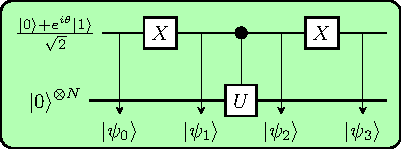
\includegraphics[width=.75\linewidth]{../circuits/circuit1}
\end{figure}
}

\begin{itemize}
\only<1>
{
	\item \(
		\ket{\psi_0} 
		= \paren{\frac{\ket 0 + e^{i\theta}\ket 1}{\sqrt 2}}\otimes \ket 0^{\otimes\elec}
		\)
	\item \(
		\ket{\psi_1}
		= \paren{\frac{\ket 1 + e^{i\theta}\ket 0}{\sqrt 2}}\otimes \ket 0^{\otimes\elec} 
		\)
	\item \(
		\ket{\psi_2}
		= \frac{\ket 1}{\sqrt 2} \otimes U \ket 0^{\otimes\elec} + \frac{e^{i\theta}}{\sqrt 2}\ket 0 \otimes \ket 0^{\otimes\elec} 
		\)
  }
	\only<1-2>
	{
	\item \(
		\ket{\psi_3}
		= \frac{\ket 0}{\sqrt 2} \otimes U \ket 0^{\otimes\elec} + \frac{e^{i\theta}}{\sqrt 2}\ket 1 \otimes \ket 0^{\otimes\elec} 
		\)
	}

	\only<2>
	{
			Changing basis on the first qubit to 
			$\ket + = \frac{\ket 0 + \ket 1}{\sqrt 2}$
			and
			$\ket - = \frac{\ket 0 - \ket 1}{\sqrt 2}$:
			\begin{equation*}
				\begin{split}
					\psi_3
					&= \frac{\ket + + \ket -}{2} \otimes U \ket 0^{\otimes\elec} + e^{i\theta}\frac{\ket + - \ket -}{2} \otimes \ket 0^{\otimes\elec} \\
					&= \ket + \frac{U + e^{i\theta}I}{2}\ket 0^{\otimes\elec}
					+ \ket - \frac{U - e^{i\theta}I}{2}\ket 0^{\otimes\elec}
				\end{split}
			\end{equation*}
	}
\end{itemize}
\end{overlayarea}
\end{frame}
\begin{frame}
	\begin{itemize}
		\item $\ket{\psi_3}
					= \ket + \frac{U + e^{i\theta}I}{2}\ket 0^{\otimes\elec}
					+ \ket - \frac{U - e^{i\theta}I}{2}\ket 0^{\otimes\elec}$
			\SubItem{The probability of measuring $\ket +$ on the first qubit is:}
\begin{equation*}
	\begin{split}
		P(\ket +)
		&= \sandwich 0 {
			\paren{\frac{U + e^{i\theta}I}{2}}
			\paren{\frac{U + e^{i\theta}I}{2}}^\dagger
		} 0 \\
		&= \frac{Re \paren{e^{i\theta}\sandwich 0 { U } 0}}{2}
		+ \frac{1}{2} \\
	\end{split}
\end{equation*}
			\SubItem{The probability of measuring $\ket -$ is then:}
\begin{equation*}
	\begin{split}
		P(\ket -)
		&= \frac{1}{2} - \frac{Re \paren{e^{i\theta}\sandwich 0 { U } 0}}{2}
	\end{split}
\end{equation*}
	\end{itemize}
\end{frame}
\begin{frame}
	\begin{itemize}
		\item Since the eigenvalue of $\ket +$ is 1 and the eigenvalue of $\ket -$ is -1, the average measurement is then:
			\SubItem{$Avg = P(\ket +) \cdot 1 + P(\ket -) \cdot (-1) = Re\paren{e^{i\theta}\sandwich 0 {U} 0}$}

		\vspace{10pt}
		\item This was a simple circuit showcasing how to obtain the expression needed. The actual circuit is larger, but uses the same general idea
\begin{equation*}
	\begin{split}
	\end{split}
\end{equation*}
	\end{itemize}
\end{frame}

\begin{frame}
\begin{figure}[ht!]
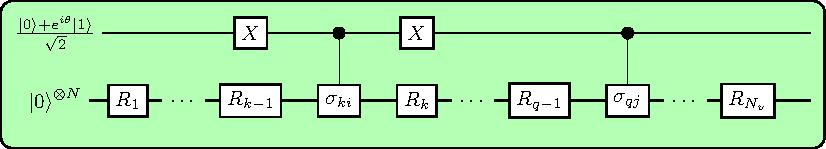
\includegraphics[width=\linewidth]{../circuits/circuit2}
\end{figure}
	\begin{itemize}
		\item Same as in the last circuit, we measure the first qubit:
\begin{equation*}
	\begin{split}
		\ket \phi
		&= \frac{\ket 0}{\sqrt 2} \otimes R_{N_v} \ldots R_k \cdot \sigma_{ki} \cdot R_{k-1} \ldots R_1 \ket 0^{\otimes \elec}\\
		&\quad + \frac{e^{i\theta}\ket 1}{\sqrt 2} \otimes R_{N_v} \ldots R_q \cdot \sigma_{qj} \cdot R_{q-1} \ldots R_1 \ket 0^{\otimes \elec}\\
		&= \frac{\ket 0}{\sqrt 2} \otimes R_{ki} \ket 0^{\otimes \elec}
		+ \frac{e^{i\theta}\ket 1}{\sqrt 2} R_{qj}\ket 0^{\otimes \elec}\\
		\span\text{Changing basis:}\\
		&= \frac{\ket + + \ket -}{2} \otimes R_{ki} \ket 0^{\otimes \elec}
		+ \frac{e^{i\theta}\paren{\ket + - \ket -}}{2} R_{qj}\ket 0^{\otimes \elec}
	\end{split}
\end{equation*}
	\end{itemize}
\end{frame}
\begin{frame}
\begin{equation*}
	\begin{split}
		\ket\phi = \ket + \otimes \frac{R_{ki} + e^{i\theta}R_{qj}}{2} \ket 0^{\otimes \elec}
		 + \ket - \otimes \frac{R_{ki} - e^{i\theta}R_{qj}}{2} \ket 0^{\otimes \elec}
	\end{split}
\end{equation*}
\begin{itemize}
	\item The probability of measuring $\ket +$ is:
\begin{equation*}
	\begin{split}
		P(\ket +)
		&= \sandwich 0 {
			\frac{1}{2}\paren{R_{ki} + e^{i\theta} R_{qj}}
			\frac{1}{2}\paren{R_{ki} + e^{i\theta} R_{qj}}^{\dagger}
		} 0 \\
		&= \frac 1 2 Re\paren{e^{i\theta}\sandwich 0 {
			 R_{ki}R_{qj}^{\dagger}
			} 0 }
			+ \frac{1}{2}\\
	\end{split}
\end{equation*}
	\item The probability of measuring $\ket -$ is then:
\begin{equation*}
	\begin{split}
		P(\ket -)
		= \frac 1 2 - \frac 1 2 Re\paren{e^{i\theta}\sandwich 0 {
			 R_{ki}R_{qj}^{\dagger}
	} 0 }
	\end{split}
\end{equation*}
\end{itemize}
\end{frame}

\begin{frame}
	\begin{itemize}
		\item The average measurement of the circuit is:
			$$Avg = P(\ket +) \cdot 1 + P(\ket -) \cdot (-1) = Re\paren{e^{i\theta}\sandwich 0 {R_{ki}R_{qj}^{\dagger}} 0}$$
		\item Taking $a_{kiqj} = \abs{if_{k, i}^*f_{q, j}}, \theta = \arg \paren{if_{k, i}^*f_{q, j}}$ and $R_{ki}R_{qj}^{\dagger}$:
\begin{equation*}
	\begin{split}
		\sum_{i, j \in P} a_{kiqj} \cdot Avg_{kiqj}
		&= \sum_{i, j \in P} a_{kiqj}\cdot Re\paren{e^{i\theta}\sandwich 0 {R_{ki}R_{qj}^{\dagger}} 0}\\
		&= \sum_{i, j \in P}
		\left [if_{k, i}^*f_{q, j}\sandwich 0 {R_{ki}R_{qj}^{\dagger}} 0 +
		H.C. \right ] \\ 
		&= M_{k, q} \\
	\end{split}
\end{equation*}
	\end{itemize}
\end{frame}

\section{\textbf{Results and Research Directions}}

\subsection{\textbf{Results}}

\begin{frame}{Error Graph - 1 electron}
\begin{figure}[b]
	\centering
	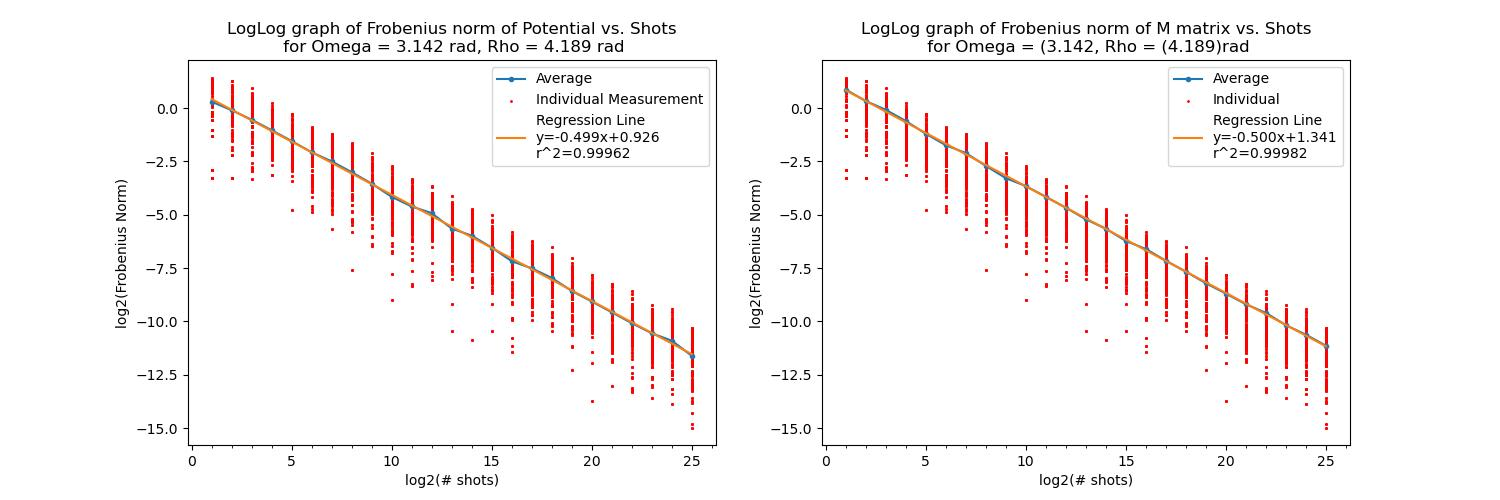
\includegraphics[width=\textwidth]{../img/1e.jpg}
  \caption{Loglog graph of error vs number of shots for a $\text{H}_2^+$ hydrogen molecule}
  \label{fig:1derrorgraph}
\end{figure}
\end{frame}

\begin{frame}{Error Graph - 2 electrons}
\begin{figure}[b]
	\centering
	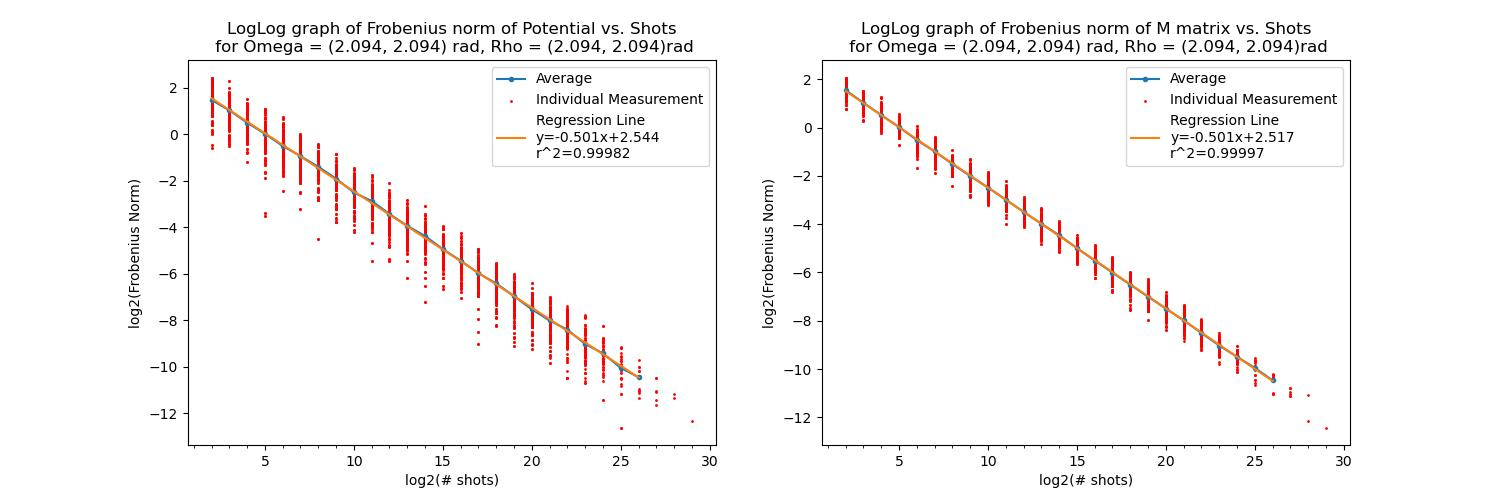
\includegraphics[width=\textwidth]{../img/2e-nonint.jpg}
  \caption{Loglog graph of error vs number of shots for a $\text{H}_2$ hydrogen molecule}
  \label{fig:2derrorgraph}
\end{figure}
\end{frame}

\subsection{\textbf{Contributions}}

\begin{frame}{Contributions}
	\begin{itemize}
		\item United HF method with other approximations to obtain a trial wavefunction for the system
		\item Decomposed said wavefunction into elementary rotations

		\item Solved the Euler-Lagrange differential equation system for specific cases so we can verify our results

		\item Further decomposed the wavefunction into a product of matrices that depend on a single variable

		\item Designed the circuit that calculates the elements of the matrices from the differential equation system

		\item Verified the theoretical output of said circuit
	\end{itemize}
\end{frame}

\subsection{\textbf{Research directions}}

\begin{frame}{Future Directions}
	\begin{itemize}
		\item Use of non-unitary representations of $\hat U$ in combination with Linear Combination of Unitaries (LCU) to make it possible to use quantum computation
		\item Apply to systems with special geometry
			\SubItem{Crystals}
			\SubItem{Polymers}
		\item Apply Quantum Approximate Optimization Algorithm (QAOA)
		\item Use Variational Quantum Eigensolver (VQE)
		\item Prepare code to submit to a real quantum computer
	\end{itemize}
\end{frame}

\begin{frame}
\frametitle{Movie Test}

Spin Density - the probability to find an electron on a infinitesimal volume $dV$

\includemovie[poster, autoplay, externalviewer, text={\small(Loading bloch.mp4)}]{6cm}{6cm}{H2.mp4}
\end{frame}

\bibliographystyle{chicago}

\section{\textbf{References}}
\bibliography{refs}

\end{document}
